\documentclass{article}
\usepackage[english]{babel}
\usepackage[utf8]{inputenc}
\usepackage{graphicx}
\usepackage{enumitem}
\usepackage{hyperref}
\usepackage{amsmath}
\usepackage{algpseudocode}
\usepackage{algorithm}

\title{Reinforcement Learning in StarCraft 2}
\author{Franz Papst}

\begin{document}
\maketitle

\section{Introduction}
Recent advances in deep reinforcement learning algorithms have successfully 
mastered the game of Go \cite{Silver2016} and are able to achieve super-human 
performance in classic Atari video games \cite{Mnih2013}. After this 
accomplishments artificial intelligence researchers are looking for a new grand 
challenge. The computer real-time strategy game StarCraft 2 seems to be a 
promising domain for research on reinforcement learning algorithms, since it 
provides a problem set that is more challenging that what was done in prior 
work. E.g. it is a multi-agent problem with multiple players interacting, it 
only give imperfect information and has a large action space \cite{Vinyals2017}.

This work is dealing with a subdomain for the whole problem set: it is about 
building an agent that is able to harvest resources as efficiently as possible. 
To solve this task I implemented an agent using the asynchronous advantage 
actor critic (A3C) algorithm \cite{Mnih2016} with TensorFlow. This report will 
firstly introduce the StarCraft 2 problem domain, by giving a detailed 
introduction into its environment. Then I will describe my agent, its 
architecture, the A3C algorithm and I implemented this algorithm. Finally I 
will analyse the performance of the agent as well as its behaviour.

\section{Environment}
The pysc2 framework\footnote{\url{https://github.com/deepmind/pysc2} verified 
2018-03-29} allows StarCraft 2 agents to be written in Python, by providing a 
Python interface for the StarCraft 2 
API\footnote{\url{https://github.com/Blizzard/s2client-api} verified 
2018-03-29}. This interface was build with reinforcement learning in mind and 
provides informations about the state of the current game, so it can be easily 
used in reinforcement learning algorithms. In the following three subsections I 
will introduce which observations are provided by the framework, how they are 
connected to states and what actions the agent can perform.

The information in this section is take from \cite{Deepmind2017} and 
\cite{Blizzard2017} or from browsing the source code myself.

\subsection{Observations}
The pysc2 framework provides the following observations:

\begin{itemize}[noitemsep]
\item \texttt{available\_actions}
\item \texttt{build\_queue}
\item \texttt{cargo}
\item \texttt{cargo\_slots\_available}
\item \texttt{control\_groups}
\item \texttt{game\_loop}
\item \texttt{minimap}
\item \texttt{multi\_select}
\item \texttt{player}
\item \texttt{score\_cumulative}
\item \texttt{screen}
\item \texttt{single\_select}
\end{itemize}

Probably the most important observations are \texttt{screen} and 
\texttt{minimap}, because the contain information about the units on screen, 
respectively on the game map. Both consist of different feature layers, as 
shown by figure \ref{screenshot}. All feature layers are two-dimensional 
arrays, containing the information similar to the pixels in an image.

\subsubsection{minimap}
A low resolution of the whole game map, it gives an overview of what's going on 
in the game, but with less detail. Initially it shows the whole map, but only 
the terrain including information about where to find resources, the position 
of the opponent is not shown, it is hidden by the so-called 
``fog-of-war''\footnote{Fog-of-war means that only those parts of the game 
world are visible where the player has a unit. If no unit is there, the 
visibility of that area slowly fades out so that only buildings remain visible, 
but no units. Changes (e.g. newly build buildings) will not be shown, until the 
player send a new unit to explore. This mechanism of the game encourages the 
player to explore the map.}. The minimap is a $(7, x,y)$ tensor, where $x$ and 
$y$ are the x- and y-resolution of the minimap. The first dimension represents 
the following features:

\begin{enumerate}[noitemsep,start=0]
\item \texttt{height\_map:} Shows the terrain level. It takes values [0,255], 
which gradually denote the height of the map, 0 being the bottom layer and 255 
being the highest elevation of the map.
\item \texttt{visibility:} Which parts of the map are hidden, have been seen or 
are currently visible. It takes values [0,1,2] denoting [hidden, have been 
seen, currently visible]
\item \texttt{creep:} Which parts of the map are covered with Zerg 
creep\footnote{One of the three races in the game, the Zerg, can only build 
buildings if the ground is covered with ``creep''. Only the command centre and 
the gas-extractor do not require to be build on creep. Creep can be extended by 
building special structures or by performing a special action for expansion. 
Zerg units move faster and regenerate when on creep, if a Zerg building is not 
surrounded by creep, it will take damage over time (apart from those buildings 
which don't need creep in the first place). This game-mechanism  emphasizes the 
organic/insect-like nature of the Zerg, as well as adding another strategical 
dimension to the game, when playing as Zerg, since it restricts where the 
player can build structures.}. It takes values [0,1] denoting denoting [no 
creep, creep].
\item \texttt{camera:} Which part of the maps is visible by the screen layer. 
It takes values [0,1] denoting [not visible, visible]
\item \texttt{player\_id:} Which player owns the units. It takes values [0,16], 
where values from 0 to 15 denote the absolute player\_id and 16 denotes neutral 
units.
\item \texttt{player\_relative:} Which status the units have relative to the 
player. It takes values [0, 1, 2, 3, 4] denoting [background, self, ally, 
neutral, hostile].
\item \texttt{selected:} Which units are selected. It takes values [0,1] 
denoting [not selected, selected].
\end{enumerate}


\subsubsection{screen}
The screen represents the visual/spatial features of the current game, similar 
to the \texttt{minimap}, showing only a part of the game map, but with a higher 
resolution. So far the screen is only represented through feature layers, but 
for future releases it is planned to add an RGB Pixel representation. Just like 
for the \texttt{minimap} also here some details are hidden by the fog-of-war, 
if there is no player unit present at the part of the map which is currently 
shown by \texttt{screen}. The screen is a $(17, x, y)$ tensor, where $x$ and 
$y$ are the x- and y-resolution of the game and the first dimension represents 
the following features:
\begin{enumerate}[noitemsep,start=0]
\item \texttt{height\_map:} The terrain level, like to \texttt{height\_level} 
from \texttt{minimap}.
\item \texttt{visibility\_map:} The visibility of the map, like 
\texttt{visibility} from \texttt{minimap}.
\item \texttt{creep:} Which parts of the screen are covered with Zerg creep, 
like \texttt{creep} from \texttt{minimap}.
\item \texttt{power:} Which parts of the screen are supplied with 
power.\footnote{Analogous to the Zerg's creep, Protoss structures need to be 
build on a part of the game map, that is supplied with power. Pylons supply the 
surrounding fields with power, meaning that other structures can be build 
there. If a pylon gets destroyed, the surrounding structures are shutting down, 
meaning being unable to operate, unless they are in reach of another pylon, 
which supplies them with energy. Like the Zerg's creep this limits the places, 
where Protoss can put structures (just like for the Zerg, this limitation does 
not apply to a command centre and a gas assimilator and also not to the pylons 
themself), making it more difficult to expand.}
\item \texttt{player\_id:} Which player owns the units on screen, like 
\texttt{player\_id} from \texttt{minimap}.
\item \texttt{player\_relative:} Which status the units on screen have relative 
to the player, like \texttt{player\_relative} from \texttt{minimap}.
\item \texttt{unit\_type:} The unit ids for all units on screen, the unit id is 
an integer from 0 to 894.\footnote{A list of unit ids can be found here: 
\url{https://github.com/Blizzard/s2client-api/blob/master/include/sc2api/sc2_typeenums.h}
 line 25ff., verified 2017-11-29.}
\item \texttt{selected:} Which units on screen are selected. It takes values 
[0,1] denoting [selected, not selected].
\item \texttt{unit\_hit\_points:} The absolute hit points the units on screen 
have. It takes values from 0, denoting no unit, to whatever value is the 
current amount of hit points for units on screen.
\item \texttt{unit\_hit\_points\_ratio:} The relative amount of hit points of 
the units on screen with respect to their maximum amount. It takes values from 
0 to 255, denoting no unit/unit destroyed or a unit with 100\% hit points.
\item \texttt{unit\_energy:} The absolute amount of energy points units on 
screen have.\footnote{Note that only some units have energy points, those are 
used to perform special actions.} It takes values from 0, denoting no 
unit/energy to whatever value is the current amount of energy for units on 
screen.
\item \texttt{unit\_energy\_ratio:} The relative amount of energy, similar to 
\texttt{unit\_hit\_points\_ratio}. It takes values from 0 to 255, denoting no 
unit/unit destroyed or a unit with 100\% hit points.
\item \texttt{unit\_shields:} The absolute amount of shield points units on 
screen have.\footnote{Note that only Protoss units have shields.} It takes 
values for 0, denoting no unit/shield points to whatever value is the current 
value of shield points for units on screen.
\item \texttt{unit\_shields\_ratio:} The relative amount of energy, similar to 
\texttt{unit\_hit\_points\_ratio}. It takes values from 0 to 255, denoting no 
unit/shield points or a unit with 100\% shield points.
\item \texttt{unit\_density:} How many units are in this pixel.
\item \texttt{unit\_density\_aa:} Like \texttt{unit\_density}, but anti-aliased 
with a maximum of 16 per unit per pixel. It shows how much of a pixel is 
covered by a unit, if multiple units are on a pixel it each proportion will be 
summed up to a value of maximum 256.
\item \texttt{effects:} Effects are the visualisation of an ongoing special 
action (e.g. healing Terran units). It takes integer values from 0 to 
3687.\footnote{A list of effect ids can be found here: 
\url{https://github.com/Blizzard/s2client-api/blob/master/include/sc2api/sc2_typeenums.h}
 line 388ff., verified 2017-11-29.}
\end{enumerate}


\subsubsection{player}
A $(11)$ tensor showing general information about the player, giving the following informations:
\begin{enumerate}[noitemsep,start=0]
\item \texttt{player\_id:} The ID of the player, an integer from 0 to 15.
\item \texttt{minerals:} Current count of minerals.
\item \texttt{vespene:} Current count of vespene gas.
\item \texttt{food\_used:} The current amount of supply used\footnote{Besides 
minerals and gas, food, also known as supply, is the third kind of resource. It 
limits how many units a player can have in total, if the current supply cap is 
reached no more new units can be produced. The maximum amount of supply is 200, 
but this does not mean, that every player can have maximum 200 units, since 
stronger units require more than 1 supply, the most supply one unit can use is 
8. In order to raise this supply cap, the player has to build special 
buildings/units depending on which race he plays.}.
\item \texttt{food\_cap:} The current maximum number of supply.
\item \texttt{food\_army:} How much of the supply is used for army units.
\item \texttt{food\_workers:} How much of the supply is used for worker units.
\item \texttt{idle\_worker\_count:} How many of the workers are currently idle.
\item \texttt{army\_count:} Current number of all army units.
\item \texttt{warp\_gate\_count:} Current number of warp gates, only for 
Protoss.
\item \texttt{larva\_count:} Current number of larva, only for Zerg.
\end{enumerate}


\subsubsection{single\_select}
A $(7)$ tensor showing information about the selected unit:
\begin{enumerate}[noitemsep,start=0]	\item \texttt{unit\_type:} The type of 
the unit.
\item \texttt{player\_relative:} Which status of the unit, relative to the 
player. It takes values [0, 1, 2, 3, 4] denoting [background, self, ally, 
neutral, hostile].
\item \texttt{health:} The current health points of the unit as absolute 
number.\footnote{Note  that just from this value it is not evident, if the unit 
is damaged or not, this information can be derived from the 
\texttt{unit\_hit\_points\_ratio} layer from the \texttt{screen} tensor.}
\item \texttt{shields:} The current shield points of the unit as absolute 
number.\footnote{Note that similar to \texttt{health} it does not give 
information about the ration of the shield to its maximum value, this 
information can be derived from the \texttt{unit\_shields\_ratio} layer from 
the \texttt{screen} tensor.}
\item \texttt{energy:} The current amount of energy points of the unit as 
absolute number.\footnote{Note that similar to \texttt{health} it does not give 
information about the ration of the shield to its maximum value, this 
information can be derived from the \texttt{unit\_energy\_ratio} layer from the 
\texttt{screen} tensor.}
\item \texttt{transport\_slot:} If the unit is transported, the amount of 
transport slots taken.
\item \texttt{build\_progress:} If the unit is being build, the percentage of 
how far the building process is.
\end{enumerate}


\subsubsection{multi\_select}
A $(n,7)$ tensor, similar to single\_select, but for $n$ selected units.


\subsubsection{build\_queue}
A $(n, 7)$ tensor, similar to \texttt{single\_select}, but for all units that 
are in the build queue of a production building, where $n$ is the number of 
units in the build queue.


\subsubsection{cargo}
A $(n, 7)$ tensor, similar to \texttt{single\_select}, but for $n$ units that are in a transporter.


\subsubsection{control\_groups}
A $(10, 2)$ tensor showing the unit leader type and count for all 10 control 
groups. A control group of units is a group that is mapped to a certain hot-key 
(0-9) in order to quickly access them.


\subsubsection{available\_actions}
A $(n)$ tensor listing all actions that are available at the time of this 
observation. The amount of total actions is quite high, but not all actions are 
available at any given point. The number $n$ of actions that are available at a 
given point in time is actually quite low. Which actions are available depends 
on what (if a) unit is selected: Some units have a lot of actions, others less 
(e.g. buildings have in general less). But there are some general actions (like 
moving the screen), which are always available.


\subsubsection{score\_cumulative}
A $(13,)$ tensor showing the ``Blizzard score''. The Blizzard score is usually 
presented to the player after the game, showing specific values of how he 
played, in order to judge how well it was:
\begin{enumerate}[noitemsep,start=0]
\item \texttt{score:} The total Blizzard score for the current step, the higher 
the better.
\item \texttt{idle\_production\_time:} Sum of the time where the player's 
production is stuck, because of reaching the supply cap, the lower the 
better.\footnote{Note that for Zerg this value does not have any meaning, since 
the way it's calculated it's always increasing.}
\item \texttt{idle\_worker\_time:} Sum of the time the player's worker units 
spend doing nothing, the lower the better.
\item \texttt{total\_value\_units:} Total sum of the value of all units the 
player built (value does not get decreased if a unit gets destroyed), the 
higher the better.
\item \texttt{total\_value\_structures:} Total sum of the value of all 
structures the player built (value does not get decreased if a structure gets 
destroyed), the higher the better.
\item \texttt{killed\_value\_units:} Total sum of all destroyed enemy 
units\footnote{Note that the value is not the same as for the 
\texttt{total\_value\_units} fields: 
\url{https://blizzard.github.io/s2client-api/sc2\_\_score\_8h\_source.html}, 
line 109f., verified 2017-11-28.}, the higher the better.
\item \texttt{killed\_value\_structures:} Total sum of all destroyed enemy 
buildings\footnote{Note that the value is not the same as for the 
\texttt{total\_value\_structures} fields: 
\url{https://blizzard.github.io/s2client-api/sc2\_\_score\_8h\_source.html}, 
line 109f., verified 2017-11-28.}, the higher the better.
\item \texttt{collected\_minerals:} Total amount of collected minerals, the 
higher the better.
\item \texttt{collected\_vespene:} Total amount of collected gas, the higher 
the better.
\item \texttt{collection\_rate\_minerals:} Current rate of mineral collection 
(minerals per minute), the higher the better.
\item \texttt{collection\_rate\_vespene:} Current rate of gas collection (gas 
per minute), the higher the better.
\item \texttt{spent\_minerals:} The total amount of minerals spent by the 
player, here it really depends which is better, in general the higher the 
better, since it correlates with a bigger, more advanced army and more workers 
(better economy).
\item \texttt{spent\_vespene:} The total amount of gas spent by the player, 
here it really depends which is better, in general the higher the better, since 
it correlates with a bigger, more advanced army.
\end{enumerate}


\subsubsection{game\_loop}
A scalar that gives the number of the current iteration in the game loop.


\subsubsection{cargo\_slots\_available}
A scalar that indicates how many cargo slots are available in a selected 
transporter.

\begin{figure}
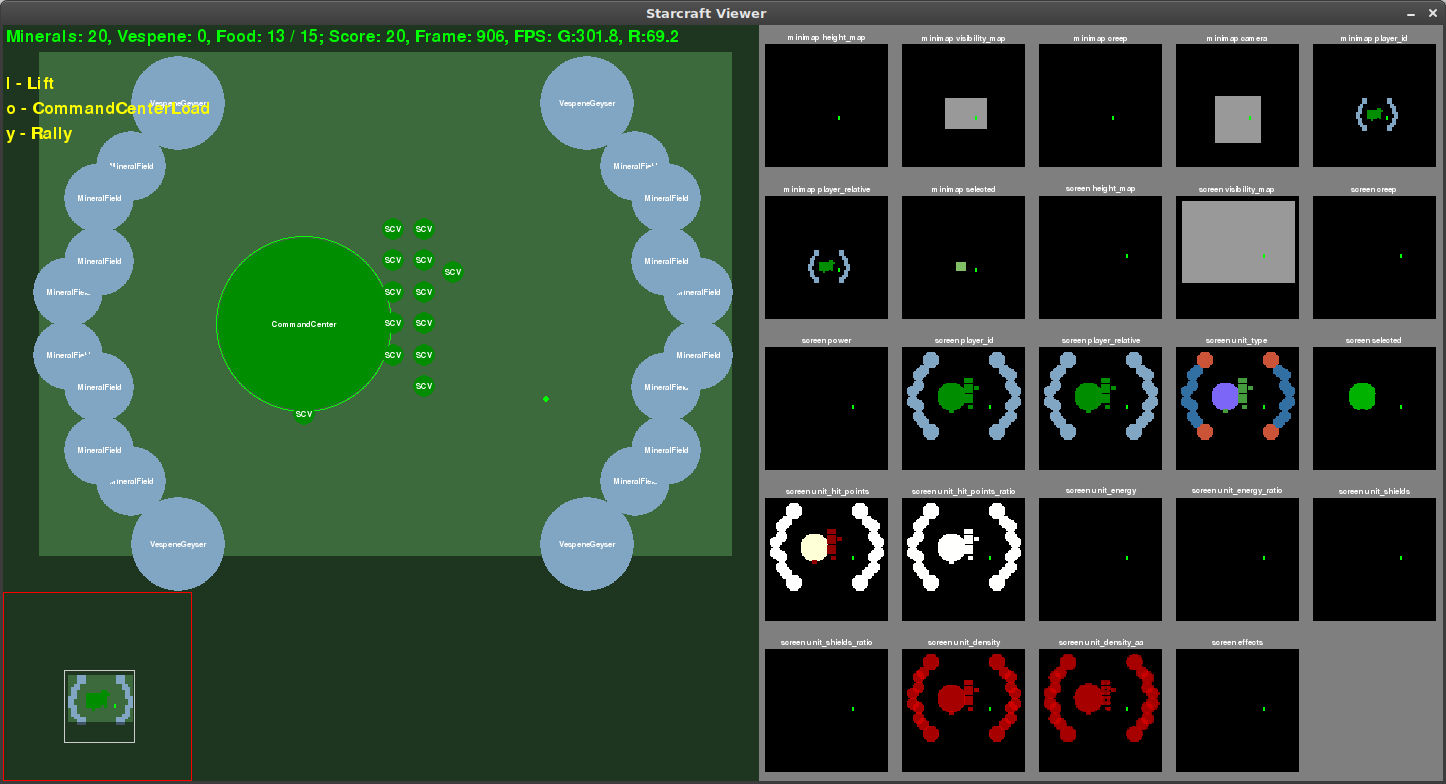
\includegraphics[width=\textwidth]{state-actions-screenshot}
\caption{Graphical representation of the different feature layers in the pysc2 
framework.}
\label{screenshot}
\end{figure}


\subsection{States}
As the exhaustive description of all observations during a single game step 
shows, the combination of possible states is huge. Therefore only the 
combination of a few features qualify to become states for the reinforcement 
learning algorithm. What makes the whole situation even more difficult is the 
fact that the action space is in general continuous, a large number of actions 
needs x- and y-coordinates where it's performed.

To reduce the agent's complexity, I will only use one of the three races for 
the beginning. I chose the Terrans, the humans, since they are usually the race 
used to teach the basics of Starcraft II. Unlike the other two races, they have 
no restrictions where they can build their structures. 

I would propose to use the following features:
\begin{itemize}[noitemsep]
\item \texttt{minimap}
\begin{itemize}[noitemsep]
	\item \texttt{visibility}
	\item \texttt{camera}
\end{itemize}
\item \texttt{screen}
\begin{itemize}[noitemsep]
	\item \texttt{player\_relative}
	\item \texttt{unit\_type}
\end{itemize}
\item \texttt{player}
\begin{itemize}[noitemsep]
	\item \texttt{minerals}
	\item \texttt{vespene}
	\item \texttt{food\_used}
	\item \texttt{food\_cap}
	\item \texttt{food\_workers}
	\item \texttt{idle\_worker\_count}
\end{itemize}
\item \texttt{score\_cumulative}
\begin{itemize}[noitemsep]
	\item \texttt{score}
	\item \texttt{idle\_worker\_time}
	\item \texttt{collected\_minerals}
	\item \texttt{collected\_vespene}
	\item \texttt{collection\_rate\_minerals}
	\item \texttt{collection\_rate\_vespene}
\end{itemize}
\item \texttt{available\_actions}
\end{itemize}

As a first naive approach all these features are fed into a simple 
multi-layer-perceptron and mapped to a one-hot encoded output. The output layer 
is a $(n, x, y)$ tensor, where $n$ is the one-hot encoded action and $x$ and 
$y$ are the x- and y-coordinates of where the action should be performed. It 
will be passed onto the agent, if an action that doesn't take any position 
arguments is performed, those arguments will be ignored from the agent.


\subsection{Actions}
As mentioned above, the action space is huge, since it is continuous. But also 
the number of different actions is rather large (in total there are 524 
different actions). The framework tackles this issue by only allowing the agent 
to execute valid actions, meaning limiting the agent to only execute actions 
that are currently available. The currently available actions can be taken from 
the \texttt{available\_actions} tensor. To keep things easy in the beginning 
only the following 15 actions will be used:

\begin{description}[noitemsep]
\item[\texttt{no\_op:}] Do nothing. It requires no target position.
\item[\texttt{move\_camera:}] Moves the camera, so it is centred around the 
target position. It requires a target position on the minimap.
\item[\texttt{select\_point:}] Selects what is at the target position (the 
action is also executed, if there is nothing at the target position, in that 
case nothing is selected). It requires a target position on the screen.
\item[\texttt{select\_rect:}] Selects all units that are within the rectangle 
that's spanned by the two target points. It requires two positions on the 
screen, where the first one is where the first click occurs (mouse button down) 
and the second one is where the drag release occurs (mouse button up).
\item[\texttt{select\_idle\_worker:}] Selects an idle worker (more or less 
randomly). It requires no target position.
\item[\texttt{Build\_CommandCenter\_screen":}] Builds a command centre. It 
requires a target position on the screen.
\item[\texttt{Build\_Refinery\_screen:}] Builds a refinery for gas on the 
screen, not that a refinery can only by build on a vespene geyser. It requires 
a target position on the screen.
\item[\texttt{Build\_SupplyDepot\_screen":}] Builds a supply depot. It requires 
a target position on screen.
\item[\texttt{Harvest\_Gather\_screen:}] Sends a worker unit to collect 
resources. It requires a target position.
\item[\texttt{Harvest\_Return\_quick:}] Makes a resource collecting worker 
unit to return the currently collected resources to base immediately. It 
requires not target position.
\item[\texttt{Morph\_SupplyDepot\_Lower\_quick:}] Lowers a supply depot, so 
it doesn't block units from passing the field it is build on. It requires 
no target position.
\item[\texttt{Morph\_SupplyDepot\_Raise\_quick:}] Raises a previously
lowered supply depot (when constructed supply depots are always raised), 
so it does prevent units from passing the field it is build on. It 
requires no target position.
\item[\texttt{Move\_screen:}] Moves units to the given position on the 
screen. It requires a target position on the screen.
\item[\texttt{Move\_minimap:}] Moves units to the given position on the 
minimap. It requires a target position on the minimap.
\item[\texttt{Rally\_Workers\_screen:}] Sets a rally point for workers on 
the screen. It requires a target position on screen.
\item[\texttt{Rally\_Workers\_minimap:}] Sets a rally point for workers on 
the minimap. It requires a target position on the minimap.
\end{description}


\section{Agent}
\subsection{Architecture}
\begin{figure}
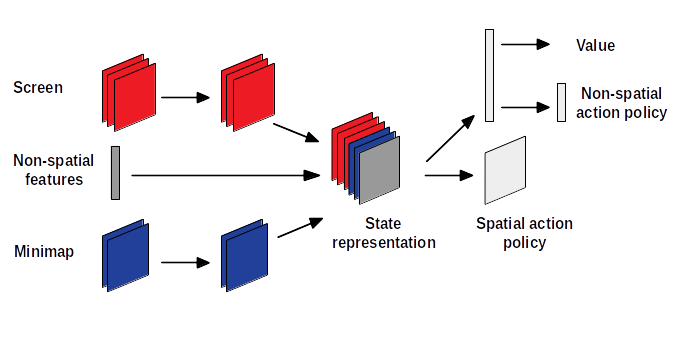
\includegraphics[width=\textwidth]{schema}
\caption{Schematic overview of the agent's architecture.}
\label{schema}
\end{figure}

Figure \ref{schema} gives a schematic overview of the agent's architecture. The 
features of screen and minimap are extracted using two convolutional neural 
networks each. As mentioned above three features from the screen and two from 
the minimap are used. The output of the last convolutional neural networks is 
concatenated with the the oupput of a fully connected neural network that was 
fed with the non-spatial inputs described above which gives the state 
representation. The state representation fed into a another convoluted neural 
network that gives the coordinates for a spatial action. The state 
representation is also fed into another fully connected neural network, which 
gives value of the current state, the same fully connected neural network is 
fed into another fully connected network that gives the non-spatial action.

The output of all neural networks is encoded in one-hot encoding, also the one 
that gives the coordinates for a spatial action. In this case the output layer 
of the neural network has a size of $x \cdot y$ and the coordinates for X and 
Y are calculated by getting the position of the highest output and performing 
an integer division by the size of $y$ for the Y-coordinate and a modulo by the 
size of $x$ for the X-coordinate.

The first convolutional neural network for the screen and the minimap has 16 
output filters, a kernel size of 5 and a stride of 1, the second one has 32 
output filters, a kernel size of 3 and a stride of 1. The fully connected 
neural network for the non-spatial features has 256 outputs with tanh as 
activation function	, the fully connected neural network for the state 
representation has 256 outputs with relu as activation function, the fully 
connected neural network for the non-spatial actions hast the number of 
available actions as output\footnote{Which is 15, as described above.} with 
softmax as activation function. The fully connected network for the value 
function has only one output and no activation function, since I am only 
interested in the value it returns.

The agent uses TensorFlow 1.5 as library for machine learning, the 
convolutional and fully connected neural networks are from the 
\texttt{contrib.layers} submodule, \texttt{contrib} features volatile and 
experimental code, \texttt{contrib.layers} features more higher level 
operations for building neural networks.

In order to be able to run the algorithm on a regular laptop\footnote{The agent 
was run on my laptop, which has an i7-7700HQ CPU, 16GB RAM, a GeForce GTX 1050 
with 4GB of VRAM.}, a few tweaks and reductions in complexity of the 
environment had to be made. The size of the screen and the minimap was reduced 
to $32 \times 32$. The agent was run in 16 parallel instances.

\subsection{Algorithm}
\label{algorithm}
The asynchronous advantage actor critic algorithm (A3C) \cite{Mnih2016} was 
used as reinforcement learning algorithm. Its advantages are its simplicity, 
its efficiency as well as its performance. It is relative easy to implement and 
resource friendly, meaning that it doesn't require specialised hardware like 
GPUs to run efficiently\footnote{When run on such specialised hardware it of 
course drastically speeds up the computation.}, but it still outperforms deep 
Q-learning on the Atari-domain and also succeeds in various continuous motor 
control tasks \cite{Mnih2016}. Previously deep reinforcement learning algorithms
had problems with stability, deep Q-learning solved this problem by introducing 
a replay buffer \cite{Mnih2013}, replay memory has the drawback of being quite 
resource consuming per real interaction Asynchronous approaches like A3C solve 
the problem of stability by introducing a parallel approach, the parallel 
execution and weight updates of different agent instances keeps the system 
stable.

A3C maintains a policy $\pi(a_t|s_t;\theta)$ and an estimate of the 
value function $V(s_t;\theta_v)$. In terms of actor-critic the policy is the 
actor and the estimate of the value function is the critic. Both get updated 
after every $t_max$ steps performed by the agent\footnote{In my implementation 
I perform an update after an episode finishes, so $t_{max} = 840$.}. The update 
of the neural network's weights can be described as $\nabla \theta' = log 
\pi(a_t | s_t; \theta') A(s_t, a_t; \theta, \theta')$, where $A(s_t, a_t; 
\theta, \theta')$ is an estimate of the advantage function given by 
$\sum_{i=0}^{k-1} \gamma^i r_{t+i} + \gamma^k V(s_{t+k}; \theta_v) - V(s_t; 
\theta)$, where $k$ is the number of the current state \footnote{In my  case 
this is equal to the number of the current step.} and is limited by $t_{max}$. 
The pseudocode for the algorithm is shown in algorithm \ref{pseudocode}.

\begin{algorithm}
\caption{Pseudocode for the asynchronous advantage actor-critic algorithm, 
taken from \cite{Mnih2016}}
\label{pseudocode}
\begin{algorithmic}
\State //Globally shared parameters: $\theta$, $\theta_v$ and counter $T = 0$
\State //Thread specific parameters: $\theta'$ and $\theta_v'$
\State Initialise thread step-counter $t \gets 1$
\Repeat
\State Reset gradients: $d\theta \gets 0$ and $d\theta \gets 0$.
\State Synchronise thread-specific parameters $\theta' = \theta$ and $\theta_v' 
= \theta_v$ 
\State $t_{start} = t$ 
\State Get state $s_t$ 
\Repeat
\State Perform $a_t$ according to policy $\pi(a_t | s_t; \theta')$
\State Receive reward $r_t$ and new state $s_{t+1}$
\State $t \gets t+1$
\State $T \gets T+1$
\Until{terminal $s_t$ or $t - t_{start} == t_{max}$}
\State R = $\begin{cases} 0 & \text{for terminal }s_t \\ V(s_t, \theta_v') & 
    \text{for non-terminal } s_t \text{//Bootstrap from last state} \end{cases}$
\For{$i \in \{t-1, \dots, t_{start}\}$}
\State $R \gets r_i + \gamma R$
\State Accumulate gradients $\theta'$: $d\theta \gets d\theta + 
    \nabla_{\theta'} log \pi(a_i | s_i; \theta') (R - V(s_i; \theta_v'))$
\State Accumulate gradients $\theta_v'$: $d\theta_v + \frac{\partial (R - 
    V(s_i; \theta_v'))^2}{\partial \theta_v'}$
\EndFor
\State Perform asynchronous update of $\theta$ using $d\theta$ and of 
    $\theta_v$ using $d\theta_v$.
\Until{$T > T{_max}$}
\end{algorithmic}
\end{algorithm}


\subsection{Implementation of the Algorithm}
\subsubsection{Agent Step}
The algorithm for updating the weights is described in section \ref{algorithm}. 
In every step the agent is fed with the above mentioned features from the 
screen, minimap and non-spatial features, in addition to the non-spatial 
features from the environment also whether the current availability from the 
executable actions is fed as input. The neural networks return the action to 
perform and the location where it should be performed. The output gets 
filtered, so that only a valid action (an action that the agent is currently 
able to do gets returned) gets passed on to the environment. During training 
there is a certain probability that the performed action is random or that the 
position where it performed is random. This level of randomness decreases 
depending on how many steps the agent has performed. The probability if an 
action is can be computed using this formula: 

\begin{equation}
P(a) = 1 - \frac{num\_steps + (1 - \epsilon_{explore}) \cdot 
T_{max}}{T_{max}}
\end{equation}

Where $\epsilon_{explore} = 0.4$ and $T_{max} = 600 \cdot 
10^6$\footnote{$T_{max}$ is the maximum amount of steps that the 
agent makes.} In addition to this adaptive probability there exists a second 
chance for an action to be random: an $\epsilon$-greedy exploration where 
$\epsilon = 0.05$. This was implemented so that the agent keeps exploring, even 
when the adaptive exploration probability reaches $0$, which happens after $240 
\cdot 10^6$ steps. The total probability of a random action is:

\begin{equation}
P(total) = P(a) + P(\epsilon)
\end{equation}

In the beginning (when $num\_steps = 0$) this would be $0.4 + 0.05 = 0.45$. The 
possibility of an position being random is computed using the same formula.

All the performed actions (with their positions) are stored, as well as the 
state for each step of the agent. The saved actions and states will be used for 
the training of the neural network as well as for logging the results of an 
episode with the actions the agent performed in this episode. In order to keep 
the size of the log files reasonable, only the actions for the top 10 episodes 
for minerals and gas, as well as the last 10 episodes are kept for every 
instance of the agent.

\subsubsection{Update of the weights}
After an episode finished, the weights of the neural networks are updated. The 
updates are done asynchronously, where each agent instance is contributing to 
the weights of the neural networks.

As described in section \ref{algorithm}, first the cumulated rewards are 
calculated. For that list of rewards is initialised with either 0, when the 
episode reached a terminal state or the reward is bootstrapped from the last 
state. From that on the lists of performed actions and states are reversed and 
the rewards get cumulated by adding the sum of the last rewards multiplied by 
the discount factor\footnote{The discount factor $\gamma$ is set to 0.99, 
because I am interested in the long term results of an action.}. By doing so 
the earlier the action took place, the higher the reward it gets assigned, 
given that the agent keeps on doing actions that give rewards. If the agent 
performs actions that decrease the rewards, also the reward decreases. The 
reward function is explained in section \ref{rewards}.

The optimiser for updating the weights is the RMSPropOptimizer \cite{RMSPROP} 
with $\epsilon = 0.1$ and $decay = 0.99$, the learning rate is variable and 
decreases the more steps the agent has performed. It can be calculated using 
the following formula:

\begin{equation}
\eta_0 \cdot \left(1 - 0.9 \cdot 
\frac{num\_steps}{T_{max}}\right)
\end{equation}

Where $\eta_0 = 10^{-3}$ and $T_{max} = 600 \cdot 10^6$.  The learning rate is 
fed into TensorFlow like an input for a neural network.

The other inputs that are fed are the states for each single step (screen, 
minimap and non-spatial features), the rewards for each single step, whether 
the selected action is spatial, which position was selected, which non-spatial 
actions are valid for the current state (this depends on which units 
are currently selected), which non-spatial action is selected and the learning 
rate. The variables for whether an action is spatial and valid non-spatial 
actions are used to create a mask for the computations of the logarithmic 
probability of an action.

One episodes consists of 840 steps, in which actions are performed\footnote{The 
execution of a map stops after 6720 steps, so for the environment it is 
actually 6720 steps, but since the agent only executed every 8th step, it only 
performs 840 actions.} In order to not need more memory for the updating of the 
weights than my GPU provides, I had to split the input data into 20 batches, 
where each includes number of 42 states, used as input.

After every 500 episodes, once the updating of the weights is done, the current 
weights are saved to hard disk.

\subsubsection{Reward Function}
\label{rewards}
\begin{equation}
minerals\ +\ gas\ \cdot\ 10\ +\ minerals\_rate\ \cdot\ 10\ +\ gas\_rate\ \cdot\ 
100
\end{equation}

The variables $minerals$ and $gas$ donate the totally collected amount of 
minerals and gas, $minerals\_rate$ and $gas\_rate$ denote the current 
collection rates of minerals and gas.

I gave gas a higher value than minerals, because minerals are rather straight 
forward to collect (the agent only has to select a worker unit and give the 
harvest command on a mineral field), while collection gas is much more 
complicated (the agent has to select a worker unit and then give a command to 
build a refinery on a specific field where a geyser is, in order to increase 
the collection rate of gas the agent can send more worker units to the build 
refinery).

I also decided to multiply the collection rate of both resources by the factor 
$10$ so that the collection rates are having significant influence on the total 
reward, also when the total collected amount of resources is already high.

\section{Results}
\subsection{Rewards}
\begin{figure}
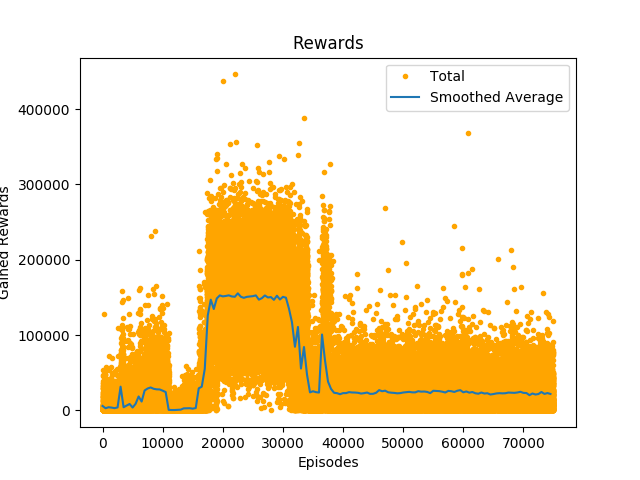
\includegraphics[width=0.75\textwidth]{rewards.png}
\caption{Gained rewards of the agent. The orange dots show the rewards of each 
single episode, the blue line shows the average of 500 episodes. The agent run 
for 75000 steps.}
\label{rewards}
\end{figure}

\begin{figure}
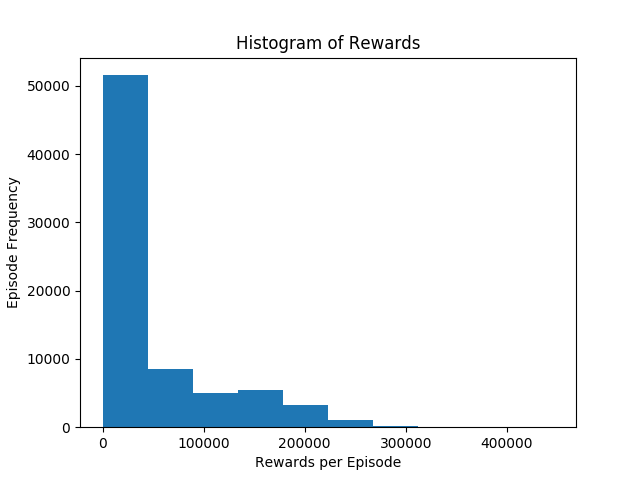
\includegraphics[width=0.75\textwidth]{rewards_histogram.png}
\caption{Histogram of rewards per episode, the histogram has 10 bins, with a 
size of 44606.4 each.}
\label{rewards_histogram}
\end{figure}

\begin{table}
\begin{tabular}{|c|c|c|c|}
\hline
Episode & Reward & Minerals & Gas\\
\hline
22104 & 446064.0 & 2345 & 468\\
19972 & 437483.9 & 1775 & 556\\
33434 & 388482.7 & 2375 & 432\\
60775 & 368278.0 & 1410 & 644\\
22227 & 356823.1 & 1315 & 452\\
32624 &  355436.2 & 1545 & 500\\
21229 &  354093.9 & 2590 & 164\\
25682 &  352979.6 & 2975 & 0\\
19094 & 340669.9 & 2930 & 0\\
32586 & 339692.5 & 3095 & 0\\
\hline
\end{tabular}
\caption{The top 10 episodes in terms of rewards.}
\label{rewards_table}
\end{table}

Figure \ref{rewards} shows all the gained rewards for every episode as well as 
the smoothed average of the rewards. Both plots show a very steep increase in 
the gained after around 15000 episodes. This lead to a plateau at a reward of 
around 150000 from around 17000 episodes to around 30000 episodes, where 
rewards were rather high in average with a few very high outliers. From 30000 
episodes to 35000 episodes the average rewards were constantly decreasing, with 
two spikes, due to very high or rather high rewards. Around 36000 episodes 
there is another spike in the average rewards, that is around 100000. From that 
on the rewards reach another plateau at around 40000 till the end. Looking at 
the plot of all rewards shows that there is a high variance in gained rewards.

Figure \ref{rewards_histogram} shows that the vast majority of episodes is in 
the first bin, meaning that they had a reward from 0 to 44606.4, this also 
shows that the agent was stuck in a plateau where the reward was around 40000 
for most of its runtime, more than 50000 episodes fall in this bin and only 
had a reward between 178425.6 and 223032 than between 133819.2 and 178425.6, 
which is not apparent from the plot of all rewards.

Table \ref{rewards_table} shows the top 10 episodes in terms of rewards. The 
top 7 episodes are episodes which are a combination of relatively high amounts 
of collected gas and high amounts of collected minerals, while in the last 
three episodes only minerals had been collected. The reason why the episode 
with a higher mineral count is because for the log files I use the last reward 
and not a sum of all rewards in an episode. By doing so, it is also visible if 
an agent performed actions that led to a decrease of the reward. This happened 
e.g. in episode 32586, where the agent started collecting minerals quickly, but 
then performed actions that didn't contribute to the increase of the reward and 
thus leading to a lower reward even though the total amount of collected 
minerals is higher than for e.g. episode 19094. Note that the final reward is 
only used for logging, for training the agent all cumulated discounted rewards 
that the agent receives are used.

\subsection{Minerals}
\begin{figure}
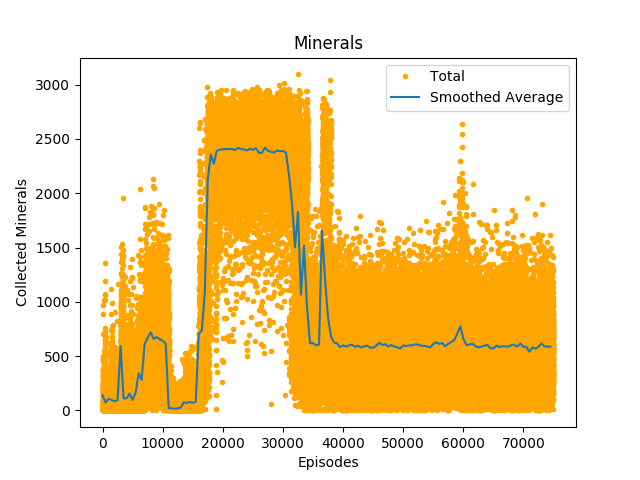
\includegraphics[width=0.75\textwidth]{minerals.png}
\caption{Collected minerals of the agent. The orange dots show the rewards of 
each single episode, the blue line shows the average of 500 episodes. The agent 
run for 75000 steps.}
\label{minerals}
\end{figure}

\begin{figure}
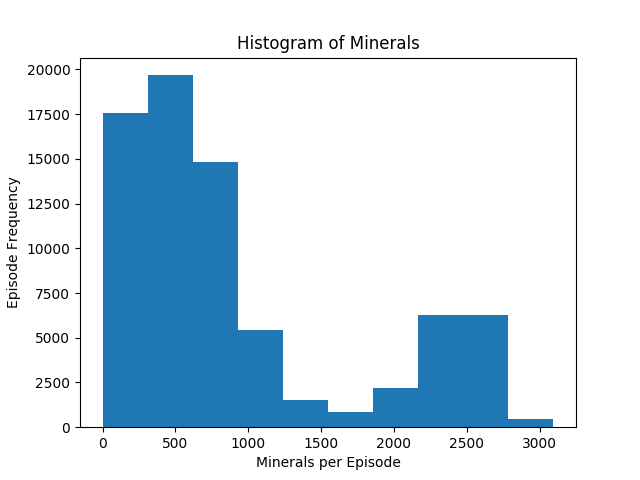
\includegraphics[width=0.75\textwidth]{minerals_histogram.png}
\caption{Histogram of collected minerals per episode, the histogram has 10 bins 
with a  size of 309.5 each.}
\label{minerals_histogram}
\end{figure}

\begin{table}
\begin{tabular}{|c|c|c|c|}
\hline
Episode & Reward & Minerals & Gas\\
\hline
32586 & 339692.5 & 3095 & 0 \\
37906 & 327749.7 & 3045 & 0 \\
30191 & 277834.5 & 3020 & 0 \\
29342 & 337969.1 & 2995 & 0 \\
17437 & 261376.8 & 2980 & 0 \\
25682 & 352979.6 & 2975 & 0 \\
30978 & 258900.1 & 2965 & 0 \\
24885 & 256661.0 & 2960 & 0 \\
30162 & 334053.1 & 2960 & 0 \\
26006 & 316695.7 & 2955 & 0 \\
\hline
\end{tabular}
\caption{The top 10 episodes in terms of collected minerals.}
\label{minerals_table}
\end{table}

Figure \ref{minerals} looks very similar to figure \ref{rewards}, indicating 
that the collected minerals are mostly responsible for the gained rewards. Also 
around 15000 episodes there is a steep rise in the amount of collected 
minerals, to slightly less than 2500 collected minerals per episode. As for the 
gained rewards, the agent stays at this plateau until around 30000 episodes, 
until it steadily decreases to around 700 collected minerals per episode until 
the end, there is also a spike around 36000 episodes, where it goes up to 
around 1000 collected minerals per episode. Around 59000 episodes there is also 
a small spike up to 800 collected minerals per episode, which does not have 
much influence on the gained rewards. Note that here the variance is also very 
high, but around the one high plateau, there are almost no very low outliers, 
meaning that during this plateau the agent practically collected minerals 
during every episode.

Figure \ref{minerals_histogram} has also some similarities to figure 
\ref{rewards_histogram}, but there is one obvious difference: the bin with the 
most episodes in is from 309.5 to 619, so there are more episodes where the 
agent collected at least 309.5 minerals than where it collected no minerals. 
Also the plateau of where the agent collects between 2476 and 2785.5 minerals  
per episode for around 14000 is easily visible in the histogram. This 
influences the slight spike in the histogram of the rewards, although since the 
influence of collected minerals on the total reward is damped, it is not so 
visible in the rewards histogram.

Table \ref{minerals_table} shows the top 10 episodes in terms of collected 
minerals. As mentioned above also here a higher amount of collected gas does 
not necessarily mean a higher amount of gained reward. It is notable that even 
though most of the top 10 episodes happened when the agent reached the highest 
plateau, the three episodes with the most collected minerals happened when the 
agent left this plateau and the are responsible for the spikes in the figure 
\ref{minerals}. Episode 17437 might be responsible for the steep increase in 
gained rewards and collected minerals that is visible in figure \ref{rewards} 
and figure \ref{minerals}, together with episodes 19972 and 19094 as shown in 
table \ref{rewards_table} because they gave very high rewards early in the 
agent's runtime.
\subsection{Gas}
\begin{figure}
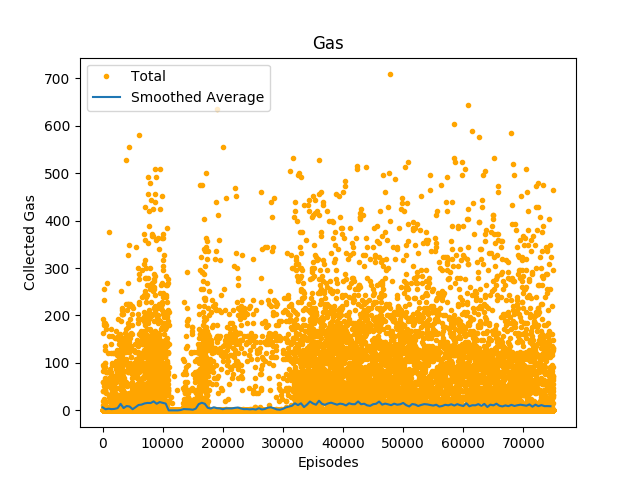
\includegraphics[width=0.75\textwidth]{gas.png}
\caption{Collected gas of the agent. The orange dots show the rewards of 
each single episode, the blue line shows the average of 500 episodes. The agent 
run for 75000 steps.}
\label{gas}
\end{figure}

\begin{figure}
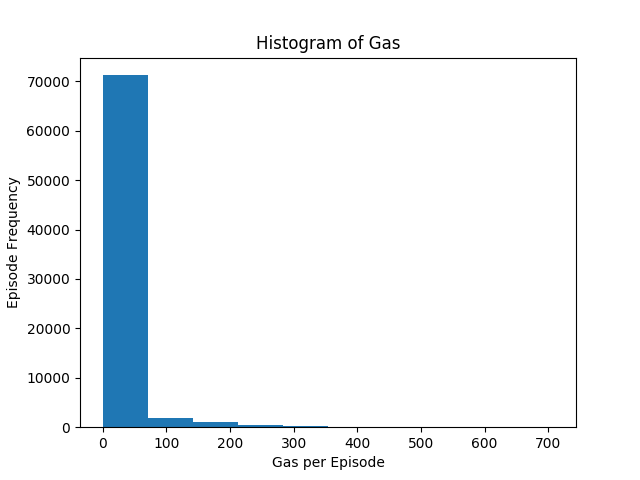
\includegraphics[width=0.75\textwidth]{gas_histogram.png}
\caption{Histogram of collected gas per episode, the histogram has 10 bins with 
a size of 70.8 each.}
\label{gas_histogram}
\end{figure}

\begin{table}
\begin{tabular}{|c|c|c|c|}
\hline
Episode & Reward & Minerals & Gas\\
\hline
47860 & 152955.0 & 760 & 708 \\
60775 & 368278.0 & 1410 & 644 \\
18985 & 334472.5 & 1595 & 636 \\
58515 & 244735.3 & 1100 & 604 \\
61472 & 187292.0 & 665 & 588 \\
67944 & 213293.6 & 915 & 584 \\
6113 & 106560.4 & 480 & 580 \\
62611 & 160610.8 & 355 & 576 \\
19972 & 437483.9 & 1775 & 556 \\
4370 & 127439.7 & 640 & 556 \\
\hline
\end{tabular}
\caption{The top 10 episodes in terms of collected gas.}
\label{gas_table}
\end{table}

Figure \ref{gas} shows how much gas an agent collected per episode, was well as 
a smoothed average. The variance is even higher than for rewards or collected 
minerals. The smoothed average is very low and usually around 0, but there are 
some very high outliers. The smoothed average is oscillating between 0 and 20 
gas collected per episode. This indicates that the agent has not learned how to 
collect gas and that the higher amounts of collected gas are the product of the 
random exploration. Looking at figure \ref{gas_histogram}, the histogram of 
collected gas, strengthens this assumption: over 70000 episodes collected 
between 0 and 70.8 gas. 

Table \ref{gas_table} shows the top 10 episodes in terms of collected gas. This 
table again highlights the rather random nature of the agent's gas collection. 
Even though collecting gas is higher valued than collecting minerals, the 
rewards of the top episodes for collected gas can not compete with the top 
episodes for collected minerals in terms of gained rewards, with the exception 
of episodes that also have a high amount of collected minerals, especially 
again episode 19972.

\subsection{Analysis of Actions}
In order to keep the file size of the logfiles reasonable only the actions for 
the top 10 episodes in terms of collected minerals and collected gas and the 
last 10 episodes where kept. For 16 agent instances this makes a maximum of 480 
episodes. In my case 468 episodes were analysed with a total of 393120 actions. 

Table \ref{total_actions} shows the frequency of all actions, table 
\ref{random_actions} shows how many of them were random and table 
\ref{non_random_actions} shows how many of them were not random. Especially 
table \ref{non_random_actions} shows that the agent learned the relation 
between performing the action ``Harvester\_Gather\_screen`` and getting a high 
reward and therefore tried to perform this action over 50\% of the time. It 
also learned that sometimes doing nothing is also beneficial for achieving this 
goal, so ``no\_op'' is the second most frequent performed action. The actions 
for selecting: ``select\_point'' and ``select\_idle\_worker'' were also learned 
from the agent, but only performed in very few cases. Taking a look at the 
action logs shows that the agent needed to perform a random select action 
before it was able to send worker units harvesting. This means that the agent 
did not learn the rule that it has to first select worker units, before it can 
send them to harvest. It is notable that the action ``select\_idle\_worker'' 
gets less often chosen by the agent than the action ``select\_point'', even 
though this action is easier to perform, since it requires no position. The 
agent was not able to learn the relation between building a refinery and 
collecting gas, since the action for building a refinery 
(``Build\_refinery\_screen'') only gets performed as random action.

The agent did not develop any particular strategy on how to maximise the amount 
of collected resources.

\subsubsection{Running the Agent on a different Map}
The trained agent was also run on different maps than the one it was trained, 
but without much success. Since the training map did not require any exploring 
of the map\footnote{It was exactly as so big that everything fitted on one 
screen.}, the agent was not really able to perform much exploration of the map 
for finding new resource patches, so it was just performing the same actions as 
it was doing on the training map, so it lead to the same results.

\begin{table}
\begin{tabular}{|l|c|}
\hline
Action & Occurrences \\
\hline
Harvest\_Gather\_screen & 53.57\% \\
no\_op & 18.073\% \\
select\_point & 5.2032\% \\
move\_camera & 5.1394\% \\
select\_idle\_worker & 3.6681\% \\
Move\_minimap & 3.3873\% \\
Move\_screen & 3.3578\% \\
Build\_Refinery\_screen & 2.2372\% \\
Build\_SupplyDepot\_screen & 1.8124\% \\
Build\_CommandCenter\_screen & 0.80255\% \\
Rally\_Workers\_screen & 0.75193\% \\
Rally\_Workers\_minimap & 0.74176\% \\
Harvest\_Return\_quick & 0.55428\% \\
Morph\_SupplyDepot\_Lower\_quick & 0.36859\% \\
Morph\_SupplyDepot\_Raise\_quick & 0.33171\% \\
\hline
\end{tabular}
\caption{Total frequency of Actions.}
\label{total_actions}
\end{table}


\begin{table}
\begin{tabular}{|l|c|}
\hline
Action & Occurrences \\
\hline
move\_camera & 5.1196\% \\
no\_op & 5.1023\% \\
select\_point & 5.0814\% \\
select\_idle\_worker & 3.6396\% \\
Harvest\_Gather\_screen & 3.4297\% \\
Move\_minimap & 3.3873\% \\
Move\_screen & 3.3578\% \\
Build\_Refinery\_screen & 2.2372\% \\
Build\_SupplyDepot\_screen & 1.8124\% \\
Build\_CommandCenter\_screen & 0.80255\% \\
Rally\_Workers\_screen & 0.75193\% \\
Rally\_Workers\_minimap & 0.74176\% \\
Harvest\_Return\_quick & 0.55428\% \\
Morph\_SupplyDepot\_Lower\_quick & 0.36859\% \\
Morph\_SupplyDepot\_Raise\_quick & 0.33171\% \\
\hline
\end{tabular}
\caption{Frequency of random Actions.}
\label{random_actions}
\end{table}

\begin{table}
\begin{tabular}{|l|c|}
\hline
Action & Occurrences \\
\hline
Harvest\_Gather\_screen & 50.141\% \\
no\_op & 12.971\% \\
select\_point & 0.12185\% \\
select\_idle\_worker & 0.02849\% \\
move\_camera & 0.019841\% \\
\hline
\end{tabular}
\caption{Frequency of non random Actions.}
\label{non_random_actions}
\end{table}

\subsection{Interpretation of the Results}
As written above, the agent was able to learn the relation between giving the 
command ``Harvester\_gather\_screen`` and an increase in reward, but the agent 
was not really able to learn the rule that it has to select a worker unit 
before it can give the harvest command. One reason for that could be that 
episodes where the ``select\_idle\_worker'' was given early on only returned 
relatively small final rewards. For example the episodes 63074, 34261 and 64866 
the ``select\_idle\_worker'' command was given quite early, but the total 
amount of collected minerals was rather low (except for episode 64866), also 
the final reward wasn't as high as one would expect. This is due to the agent 
ordering the worker units to harvest early on, but then gives other commands, 
which keeps them from harvesting. Another special case is episode 37906, it was 
the second best episode in terms of collected minerals and also the reward was 
quite high. In this episode the agent didn't give much ``useless'' commands, 
that kept the worker units from collecting minerals. The reason why I was only 
looking at the ``select\_idle\_worker'' command is, because there it is more 
likely that the agent actually selects a worker unit, for select point this can 
not be said, since the agent could also select a random point and so selects no 
unit.

The agent not learning the relation between selecting a worker unit before it 
can give the harvesting command also explains why the agent wasn't able to 
learn how to collect gas. In order to collect gas it had to also learn the 
relation between building a refinery at the right position, something it also 
didn't do.

The agent performing some select actions, and especially that those actions 
were performed rather early, indicate that the agent would have been able to 
learn this correlations, if given more time. After 75000 episodes the agent was 
stuck in a local minima and the average rewards as well as the average 
collected minerals per episode were plateauing. It is difficult to say, how 
long this plateau would have lasted, but given that the agent reached a higher 
plateau before it is likely that the agent would have left that local minima.

\section{Conclusion}
Running and observing the behaviour of the agent leads to the conclusion, that 
the state space of StarCraft II is so large, that it can not be efficiently 
explored by a reinforcement learning algorithm without specialised hardware, 
even though with the A3C algorithm a reinforcement learning algorithm that is 
known to have rather low resource demands was chosen.

The agent showed some ``intelligent'' behaviour, especially since it learned 
the relation between harvesting resources and an increase in reward. From the 
action logs of the agent however it is obvious that the agent did not learn 
that it had to select a worker unit before it can give the command to harvest 
minerals nor did it learn how to harvest gas. The data from the action logs 
however also suggests that the agent could learn the relation of selecting a 
worker unit before it can give the harvesting command, if it is trained for a 
longer time.

Two things that possibly could speed up this convergence process are using the 
\texttt{single\_select} tensor as input as well as performing an update after 
$n$ steps instead of after every episode. The former would give the agent a 
more direct feedback whether a select action was successful (so far this 
feedback is only given indirectly by whether more actions become available), 
while the latter would make improvements in the action policy faster available 
to the agent.

Another possibility would have been to give the agent more guidance in the 
learning process. It might would have made the agent faster in solving the 
task, but it would also required more intervention from my side and would 
override one big advantage of reinforcement learning: that the agent is able to 
find a solution with little to no prior knowledge build into it.


\begin{thebibliography}{alpha}
\bibitem{Vinyals2017} Vinyals, Oriol, et al. "StarCraft II: A New Challenge for 
Reinforcement Learning." \emph{arXiv preprint arXiv:1708.04782} (2017).

\bibitem{Mnih2013} Mnih, Volodymyr, et al. "Playing atari with deep 
reinforcement learning", \emph{arXiv preprint arXiv:1312.5602} (2013).

\bibitem{Mnih2016} Mnih, Volodymyr, et al. "Asynchronous methods for deep 
reinforcement learning." \emph{International Conference on Machine Learning}. 
2016.

\bibitem{Hinton2014} Hinton, G. et al. "Lecture 6a Overview of Mini-Batch 
Gradient Descent." \emph{Lecture Notes Distributed in CSC321 of University of 
Toronto.} 2014. Available online: 
\url{http://www.cs.toronto.edu/~tijmen/csc321/slides/lecture_slides_lec6.pdf} 
verified 2018-03-29.

\bibitem{Silver2016} Silver, David, et al. "Mastering the game of Go with deep 
neural networks and tree search." \emph{Nature} 529.7587 (2016): 484-489.

\bibitem{Deepmind2017} DeepMind Technologies Limited. "PySC2 - StarCraft II 
Learning Environment" \emph{GitHub} 2017. Available online: 
\url{https://github.com/deepmind/pysc2/blob/master/docs/environment.md} 
verified 2018-03-29.

\bibitem{Blizzard2017} Blizzard Entertainment, Inc. "SC2API Documentation" 
\emph{GitHub} 2017. Available online: 
\url{https://blizzard.github.io/s2client-api/}, verified 2018-03-29.

\end{thebibliography}

\end{document}
